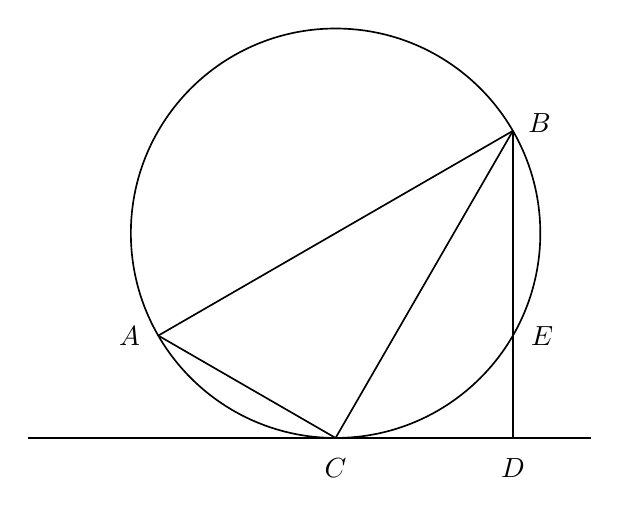
\begin{tikzpicture}[x=1cm,y=1cm,line width=.6pt,font=\normalsize]
\coordinate (O) at (0,0);
\coordinate (A) at (-2.2516,-1.3);
\coordinate (B) at (2.2516,1.3);
\coordinate (C) at (0,-2.6);
\coordinate (D) at (2.2516,-2.6);
\coordinate (E) at (2.2516,-1.3);
\coordinate (T1) at (-3.9,-2.6);
\coordinate (T2) at (3.25,-2.6);
\draw (O) circle[radius=2.6cm];
\draw (A)--(B);
\draw (A)--(C);
\draw (B)--(C);
\draw (B)--(E)--(D);
\draw (T1)--(T2);
\node[left=3pt] at (A) {$A$};
\node[below=4pt] at (C) {$C$};
\node[above=3pt,right=2pt] at (B) {$B$};
\node[below=4pt] at (D) {$D$};
\node[right=3pt] at (E) {$E$};
\end{tikzpicture}
